% =====================================================================================================
% vygotskian_cortex.tex — The Vygotskian machine, part 2: the CORTEX architecture it is built on
%
% DRAFT (2026-11-20, cut to budget). Describes what exists today, as a given resource. Descriptive, not a report
% of results: every component named here is in the robocomp/active_inference repository (ARCHITECTURE.md is the
% source). Include after vygotskian_machine.tex and before vygotskian_internalisation.tex.
% =====================================================================================================

\section{The Starting Point: the CORTEX Architecture}
\label{sec:cortex}

The Vygotskian machine is added to an existing and working robot architecture, \cortex{}, which runs on a mobile
robot called Shadow, both in a simulated apartment and in a real one. \cortex{} already builds a probabilistic model of
the robot's surroundings, acts on that model, remembers it, and talks about it with a person
through a language agent. We describe the architecture as it stands, because each proposal in the later sections is
defined by what it adds to these parts.

% CORTEX architecture overview, extended for the Vygotskian machine paper (2026-11-20).
% Derived from the Autonomous Robots paper's fig:overview. Changes: a LANGUAGE LEVEL band on top, where the language
% agent is drawn in its full role (outer speech = exists today, solid; inner voice + cultural plane = added by this
% paper, dashed); the old small language-agent box became the command gate it acts through; a level-4 function agent
% (dashed) joins the concept column; the concept column was respaced to make room for it.
% Needs: tikz (arrows.meta, positioning, shapes.geometric, calc, shadows), adjustbox, and the colours + \cortex
% defined in vygotskian_machine_build.tex.
\begin{figure*}[!tp]
\centering
\begin{adjustbox}{max width=\textwidth}
\begin{tikzpicture}[
  >=Latex, font=\small,
  ag/.style={rounded corners=3pt, thick, align=center, minimum width=26mm, minimum height=8.5mm, inner sep=2pt},
  concept/.style={ag, draw=conceptc, fill=conceptf, text=conceptc!80!black},
  stack/.style={concept, double copy shadow={shadow xshift=1.2pt, shadow yshift=1.2pt, draw=conceptc, fill=conceptf}},
  mem/.style={ag, draw=memc, fill=memf, text=memc!80!black},
  lang/.style={ag, draw=langc, fill=langf, text=langc!80!black},
  langnew/.style={ag, draw=langc, dashed, very thick, fill=white, text=langc!80!black, minimum width=38mm, minimum height=17mm},
  langold/.style={ag, draw=langc, very thick, fill=white, text=langc!80!black, minimum width=38mm, minimum height=17mm},
  body/.style={ag, draw=bodyc, fill=bodyf, text=bodyc!70!black},
  drv/.style={rectangle, rounded corners=2pt, draw=bodyc!70, fill=white, thick, align=center, font=\footnotesize, minimum width=19mm, minimum height=7mm},
  dev/.style={rectangle, rounded corners=2pt, draw=gray!60, fill=gray!10, align=center, font=\footnotesize, minimum width=19mm, minimum height=6mm},
  wmlink/.style={{Latex[length=2.2mm]}-{Latex[length=2.2mm]}, very thick, draw=arrowc!80},
  stream/.style={-{Latex[length=2.2mm]}, very thick, draw=azuloscuro!80},
  cmd/.style={-{Latex[length=2.2mm]}, very thick, draw=cmdc},
  langarrow/.style={-{Latex[length=2.2mm]}, very thick, draw=langc},
  mini/.style={circle, inner sep=0pt, minimum size=2.6mm, draw=black!70},
  rt/.style={-{Latex[length=1.3mm]}, draw=black!60},
  lvl/.style={font=\bfseries\large, text=black!70, anchor=north west}]
% ---------- backgrounds
\fill[langf!70, rounded corners=10pt] (-8.4,5.0) rectangle (8.4,9.75);
\node[lvl] at (-8.25,9.7) {LANGUAGE LEVEL \normalfont\normalsize --- the Vygotskian machine};
\fill[wmf!60, rounded corners=10pt] (-8.4,-4.25) rectangle (8.4,4.6);
\node[lvl, anchor=west] at (-8.25,-1.75) {COGNITIVE LEVEL};
\fill[bodyf!50, rounded corners=10pt] (-8.4,-9.2) rectangle (8.4,-5.95);
\node[lvl] at (-8.25,-6.15) {SUB-COGNITIVE LEVEL};
% ---------- language level: the language agent in its full role
\node[draw=langc, very thick, rounded corners=6pt, fill=langf, minimum width=128mm, minimum height=37mm] (lab) at (1.2,7.15) {};
\node[font=\bfseries, text=langc, anchor=north] at (1.2,8.95) {Language agent \normalfont\footnotesize(VLM on the Orin, proposes; the robot's models dispose)};
\node[langold] (os) at (-3.0,7.0) {\textbf{Outer speech}\\[-1pt]{\scriptsize chat, missions, approval}\\[-2pt]{\scriptsize wake turns, ask or assume}};
\node[langnew] (iv) at (1.2,7.0)  {\textbf{Inner voice}\\[-1pt]{\scriptsize self-addressed questions}\\[-2pt]{\scriptsize demand $\to$ attention modes}};
\node[langnew] (cp) at (5.4,7.0)  {\textbf{Cultural plane}\\[-1pt]{\scriptsize culture: function priors}\\[-2pt]{\scriptsize sequencing $\cdot$ imagination}};
\draw[-{Latex[length=1.8mm]}, thick, draw=langc!80] (os) -- (iv);
\draw[-{Latex[length=1.8mm]}, thick, draw=langc!80] (iv) -- (cp);
\node[font=\scriptsize, text=langc!80!black, anchor=north east] at (8.3,9.68) {solid: exists in \cortex{} $\cdot$ dashed: added by this paper};
\node[ag, draw=black!60, fill=white, text=black, minimum width=17mm] (person) at (-7.15,8.1) {Person};
\draw[{Latex[length=2.2mm]}-{Latex[length=2.2mm]}, very thick, draw=langc] (person.east) -- node[above, font=\tiny, text=langc] {speech} (person.east -| lab.west);
\node[ag, draw=langc, dashed, fill=white, text=langc!80!black, minimum width=20mm, font=\footnotesize] (imw) at (-7.15,6.15) {Imagined world\\[-1pt]{\tiny copy; never writes WM}};
\draw[{Latex[length=1.8mm]}-{Latex[length=1.8mm]}, thick, draw=langc] (imw.east) -- node[above, font=\tiny, text=langc] {imagine} (imw.east -| lab.west);
% ---------- working memory with a miniature graph
\node[ellipse, draw=wmc, very thick, fill=wmf, minimum width=72mm, minimum height=44mm] (wm) at (0,0) {};
\node[font=\bfseries, text=wmc] at (0,1.8) {Working memory};
\node[font=\scriptsize, text=wmc!80, align=center] at (2.15,-1.35) {replicated\\graph of beliefs};
\node[mini, fill=black] (root) at (-0.3,-1.5) {};  \node[font=\tiny, right] at (root.east) {root};
\node[mini, fill=wmc!40] (room) at (-0.3,-0.9) {};  \node[font=\tiny, right] at (room.east) {room};
\node[mini, fill=bodyc!60] (rob) at (0.7,-0.35) {};  \node[font=\tiny, right] at (rob.east) {robot};
\node[mini, fill=bodyc!35] (bod) at (0.7,0.3) {};    \node[font=\tiny, right] at (bod.east) {body};
\node[mini, fill=orange] (cam) at (-0.1,0.85) {};      \node[font=\tiny, left] at (cam.west) {camera};
\node[mini, fill=yellow!80!black] (lid) at (0.7,1.0) {}; \node[font=\tiny, above] at (lid.north) {LiDAR};
\node[mini, fill=brown!70] (imu) at (1.5,0.85) {};    \node[font=\tiny, right] at (imu.east) {IMU};
\node[mini, fill=conceptc!50] (door) at (-2.3,-0.55) {}; \node[font=\tiny, left] at (door.west) {door};
\node[mini, fill=conceptc!50] (tab) at (-1.45,0.25) {}; \node[font=\tiny, left] at (tab.west) {table};
\node[mini, fill=white, draw=conceptc] (aff) at (-1.45,0.95) {}; \node[font=\tiny, left] at (aff.west) {offer};
\node[mini, fill=conceptc!50] (hum) at (2.3,-0.6) {}; \node[font=\tiny, right] at (hum.east) {person};
\draw[rt] (root) -- (room); \draw[rt] (room) -- (rob); \draw[rt] (rob) -- (bod);
\draw[rt] (bod) -- (cam); \draw[rt] (bod) -- (lid); \draw[rt] (bod) -- (imu);
\draw[rt] (room) -- (door); \draw[rt] (room) -- (tab); \draw[rt] (room) to[bend right=15] (hum);
\draw[-{Latex[length=1.3mm]}, densely dashed, draw=conceptc] (tab) -- (aff);
\node[font=\tiny, text=black!55] at (0.2,-1.25) {RT};
% ---------- memories (left)
\node[mem] (ltsm) at (-6.15,2.75) {LTSM\\[-1pt]{\scriptsize rooms, passages; own graph}};
\node[mem] (em)   at (-6.15,1.15) {Episodic memory\\[-1pt]{\scriptsize commitments, effects}};
\node[mem] (ltom) at (-6.15,-0.45) {LTOM\\[-1pt]{\scriptsize individuals, names}};
% ---------- concepts (right); the function agent (level 4) is this paper's addition
\node[concept, draw=langc, dashed, very thick, text=langc!80!black] (fn) at (6.15,3.3) {Function (level 4)\\[-1pt]{\scriptsize room purpose}};
\node[concept] (mc)  at (6.15,2.25)  {Meta-concepts\\[-1pt]{\scriptsize dining set, kitchen}};
\node[concept] (rc)  at (6.15,1.2)   {Room concept\\[-1pt]{\scriptsize localiser, outline}};
\node[stack]   (dc)  at (6.15,0.15)  {Door concept};
\node[stack]   (oc)  at (6.15,-0.9)  {Object concepts\\[-1pt]{\scriptsize table, chair, cabinet, \ldots}};
\node[stack]   (hc)  at (6.15,-1.95) {Human concept};
\node[concept] (res) at (6.15,-3.0)  {Residual\\[-1pt]{\scriptsize null hypothesis}};
% ---------- top of cognitive level: the gate the language agent acts through, and self-calibration
\node[lang] (gate) at (-2.6,3.8) {Command gate\\[-1pt]{\scriptsize checks names, plans, capabilities}};
\node[body] (sc) at (3.1,3.8) {Self-calibration\\[-1pt]{\scriptsize body beliefs}};
% ---------- bottom of cognitive level: the bridge
\node[body] (rbc) at (-3.6,-3.55) {Robot concept\\[-1pt]{\scriptsize frame tree, bridge}};
\node[body] (ret) at (0,-3.55)    {Retina\\[-1pt]{\scriptsize DNNs $\to$ likelihoods}};
\node[body] (ctl) at (3.6,-3.55)  {Controller\\[-1pt]{\scriptsize ranks offers by $G$}};
% ---------- links to the working memory
\foreach \n in {ltsm,em,ltom} \draw[wmlink] (\n.east) -- (wm);
\foreach \n in {fn,mc,rc,dc,oc,hc,res} \draw[wmlink] (\n.west) -- (wm);
\foreach \n in {gate,sc,rbc,ret,ctl} \draw[wmlink] (\n) -- (wm);
% ---------- language level <-> cognitive level
\draw[langarrow] (gate.north |- lab.south) -- node[left, font=\tiny, text=langc, align=right, pos=0.4] {proposals:\\missions, tool calls} (gate.north);
\draw[langarrow, densely dashed] (0.9,2.13) -- node[left, font=\tiny, text=langc, align=right, pos=0.78] {beliefs + prediction\\error $\to$ demand} (0.9,0 |- lab.south);
\draw[{Latex[length=2mm]}-{Latex[length=2mm]}, thick, draw=langc!70, densely dashed] (-5.05,0 |- lab.south) -- node[left, font=\tiny, text=langc, align=right, pos=0.45] {tools: memories,\\counts} (-5.05,0 |- ltsm.north);
\draw[-{Latex[length=2mm]}, thick, draw=langc, dashed] (lab.east |- cp) -| (8.05,3.3) -- (fn.east);
\node[font=\tiny, text=langc, rotate=90, anchor=north] at (8.1,5.2) {elicited priors};
% ---------- media plane
\node[rectangle, draw=azuloscuro, very thick, fill=azuloscuro!8, minimum width=164mm, minimum height=8mm, align=center] (mp) at (0,-5.15)
  {\textbf{\textcolor{azuloscuro}{Media plane}}\quad{\footnotesize own DDS domain $\cdot$ shared memory $\cdot$ zero-copy $\cdot$ descriptors on sensor nodes}};
\draw[stream] (mp.north -| ret) -- (ret.south);
\draw[stream] (mp.north -| ctl) ++(-0.6,0) -- ++(0,0.98);
\draw[stream] (mp.north -| rbc) ++(0.6,0) -- ++(0,0.98) node[midway, right, font=\tiny, text=azuloscuro] {};
\draw[stream] (7.85,-4.75) |- node[pos=0.25, right, font=\tiny, text=azuloscuro] {LiDAR} (res.east);
% ---------- drivers and devices
\node[drv] (d1) at (-6.2,-7.3) {stereo\\[-2pt]camera};
\node[drv] (d2) at (-3.7,-7.3) {360$^\circ$\\[-2pt]camera};
\node[drv] (d3) at (-1.2,-7.3) {LiDAR\\[-2pt]upper};
\node[drv] (d4) at (1.3,-7.3)  {LiDAR\\[-2pt]lower};
\node[drv] (d5) at (3.8,-7.3)  {IMU};
\node[drv] (d6) at (6.3,-7.3)  {base};
\foreach \d in {d1,d2,d3,d4,d5} \draw[stream] (\d.north) -- (\d.north |- mp.south);
\node[dev] (e1) at (-6.2,-8.55) {ZED};   \node[dev] (e2) at (-3.7,-8.55) {Ricoh};
\node[dev] (e3) at (-1.2,-8.55) {Helios}; \node[dev] (e4) at (1.3,-8.55) {Bpearl};
\node[dev] (e5) at (3.8,-8.55) {IMU 9DoF}; \node[dev] (e6) at (6.3,-8.55) {motors};
\foreach \i in {1,...,6} \draw[{Latex[length=1.6mm]}-{Latex[length=1.6mm]}, thick, gray!60] (e\i) -- (d\i);
\draw[cmd] ([xshift=9mm]ctl.south) |- (5.6,-4.5) -| node[pos=0.88, left, font=\tiny, text=cmdc, align=right] {velocity\\commands} (d6.north);
\node[font=\scriptsize, text=bodyc!80!black, anchor=west] at (-8.3,-7.95) {drivers};
\node[font=\scriptsize, text=gray, anchor=west] at (-8.3,-9.0) {devices};
\end{tikzpicture}
\end{adjustbox}
\caption{The \cortex{} architecture with the Vygotskian machine on top. At the cognitive level, every process is a
peer of the working memory (centre), the replicated graph of beliefs whose miniature shows the robot's frame tree, the
room with its concepts, a person and an offer. Concept agents (blue; stacked boxes own many instances) and memory
agents (green) read and write it, and each memory agent keeps a graph of its own on the same distributed substrate.
The robot concept, retina, controller and self-calibration (red) connect beliefs to the body: sensor streams rise on
the media plane (blue arrows) and velocity commands go down to the base (red). Teal arrows are reads and writes of the
working memory. The language level (violet) is the language agent in the role this paper gives it. Its outer speech
--- chat with the person, missions the person approves, restricted wake turns --- exists in \cortex{} today; the inner
voice and the cultural plane (dashed) are added by this paper (Sections~\ref{sec:inner_speech}
and~\ref{sec:lang_hierarchy}). Everything it proposes reaches the working memory only through the command gate; it
reads beliefs, memories and counts, imagines on a copy of the world that cannot write the graph, and is recruited by a
demand signal computed from the prediction errors of the levels below. Culture reaches the belief hierarchy as priors
of the new level-4 function agent (dashed), elicited offline, never as beliefs.}
\label{fig:cortex_overview}
\end{figure*}


\paragraph{A shared graph of beliefs.}
At its core, \cortex{} is a shared, distributed and persistent scene graph, read and written concurrently by independent
processes called agents (Figure~\ref{fig:cortex_overview}, where the graph is drawn as the working memory). Agents
do not send messages to one another, and the graph
is the only interface through which they communicate. Each agent keeps a full replica, and the replicas are merged as
conflict-free replicated data types, whose copies converge to the same state without coordination. Geometric edges
hold a rigid transform with its covariance, and they form a tree from the world through the rooms to the objects, and
from the robot's base to its sensors. An agent is a process that maintains a probabilistic belief over one kind of
entity and publishes it with its mean and covariance. Other agents treat this posterior as evidence weighted by its
covariance, and never as ground truth. Effects that a conventional system would express as a threshold, such as
ignoring distant detections, are instead written into the generative model, usually as a covariance that grows with a
physical quantity. The thresholds that this paper does introduce are declared, with their justification, in
Section~\ref{sec:inner_speech:modes}.

\paragraph{A probabilistic hierarchy.}
The beliefs in the graph form a hierarchy of five levels (Table~\ref{tab:lh_levels}), namely the robot itself, its
rooms, the objects in those rooms, aggregates of objects, and cultural abstractions such as what a room is for. Each
level is expressed in the frame of the level below, its measurements are the posteriors published by that level, and
it can send back down an empirical prior, that is, a message stating what it expects its parts to be. The first four
levels constitute \cortex{} as it exists, and they are built automatically and without language. The fifth is the
addition made in this paper. Figure~\ref{fig:cortex_graph} shows the graph that \cortex{} builds in the simulated
apartment.

\begin{table}[ht]
    \centering
    \small
    \begin{tabular}{|>{\raggedright\arraybackslash}p{0.05\linewidth}|>{\raggedright\arraybackslash}p{0.16\linewidth}|>{\raggedright\arraybackslash}p{0.33\linewidth}|>{\raggedright\arraybackslash}p{0.17\linewidth}|>{\raggedright\arraybackslash}p{0.13\linewidth}|}
        \hline
        \textbf{Level} & \textbf{What} & \textbf{Latent} & \textbf{Source of its model} & \textbf{Status} \\ \hline
        0 & robot (self) & body, sensor mounts, pose & calibration, self-calibration & implemented \\ \hline
        1 & room(s) & layout of each room, the robot's place in it, the doors that join rooms & authored generative model, fitted online; spatial memory & implemented \\ \hline
        2 & objects & per instance: class, pose, extent, existence & authored generative models, fitted online & implemented \\ \hline
        3 & metaconcepts (aggregates) & arrangements: a ring of chairs around a table, the rectilinear frame of a kitchen & authored schemas & implemented (the kitchen's priors not yet sent down) \\ \hline
        4 & cultural abstraction & the function of a room (kitchen, dining, bedroom, \ldots) & \textbf{culture: the VLM}, weighted by measured reliability and replaced by counts & \textbf{added by this paper} (Section~\ref{sec:lang_hierarchy:culture}) \\ \hline
    \end{tabular}
    \caption{The probabilistic belief hierarchy. Levels 0--3 are \cortex{} as it exists, and level 4 is added here.}
    \label{tab:lh_levels}
\end{table}



\paragraph{Levels 0 to 3.}
At level 0, an agent dedicated to the body maintains the tree of frames from the base to each sensor, and a
self-calibration agent estimates where each sensor is mounted, so that these transforms are themselves beliefs. At
level 1, a room agent jointly estimates the layout of the current room and the robot's location in it, and decides
from evidence whether the robot has entered a new room or returned to a known one. Rooms are joined by doors, and the
robot's world is a graph of rooms of which only one is actively estimated at a time. At level 2, each class of object
has its own concept agent, for tables, chairs, cabinets, refrigerators, doors, beds, people and others. Each agent
tracks instances from segmentation masks and depth, updates a class-specific generative model with a shared recursive
variational Laplace engine, and publishes each instance in the frame of its room. A residual agent models the
occupancy that no other agent explains, and acts as the null hypothesis of the scene. Every instance carries an
existence log-odds, raised by evidence that was predicted and observed and lowered by evidence that was predicted but
absent, only where the object could have been detected, so that an occluded object is retained rather than refuted.
At level 3, two metaconcepts fit aggregates, a table with its ring of chairs and the frame shared by the units of a
kitchen. The existence of an aggregate is a log Bayes factor against an explicit null of independent objects, and
each aggregate sends empirical priors to its members, computed without that member's own contribution
(Eq.~\eqref{eq:lh_cavity}). Level 4, the purpose of a room and how the robot should behave there, is not represented
in \cortex{} and is the contribution of this paper (Section~\ref{sec:lang_hierarchy:culture}).



\begin{figure}[!h]
    \centering
    \begin{minipage}[c]{0.53\linewidth}
        \centering
        \begin{tikzpicture}
            \node[anchor=south west, inner sep=0] (img) at (0,0)
                {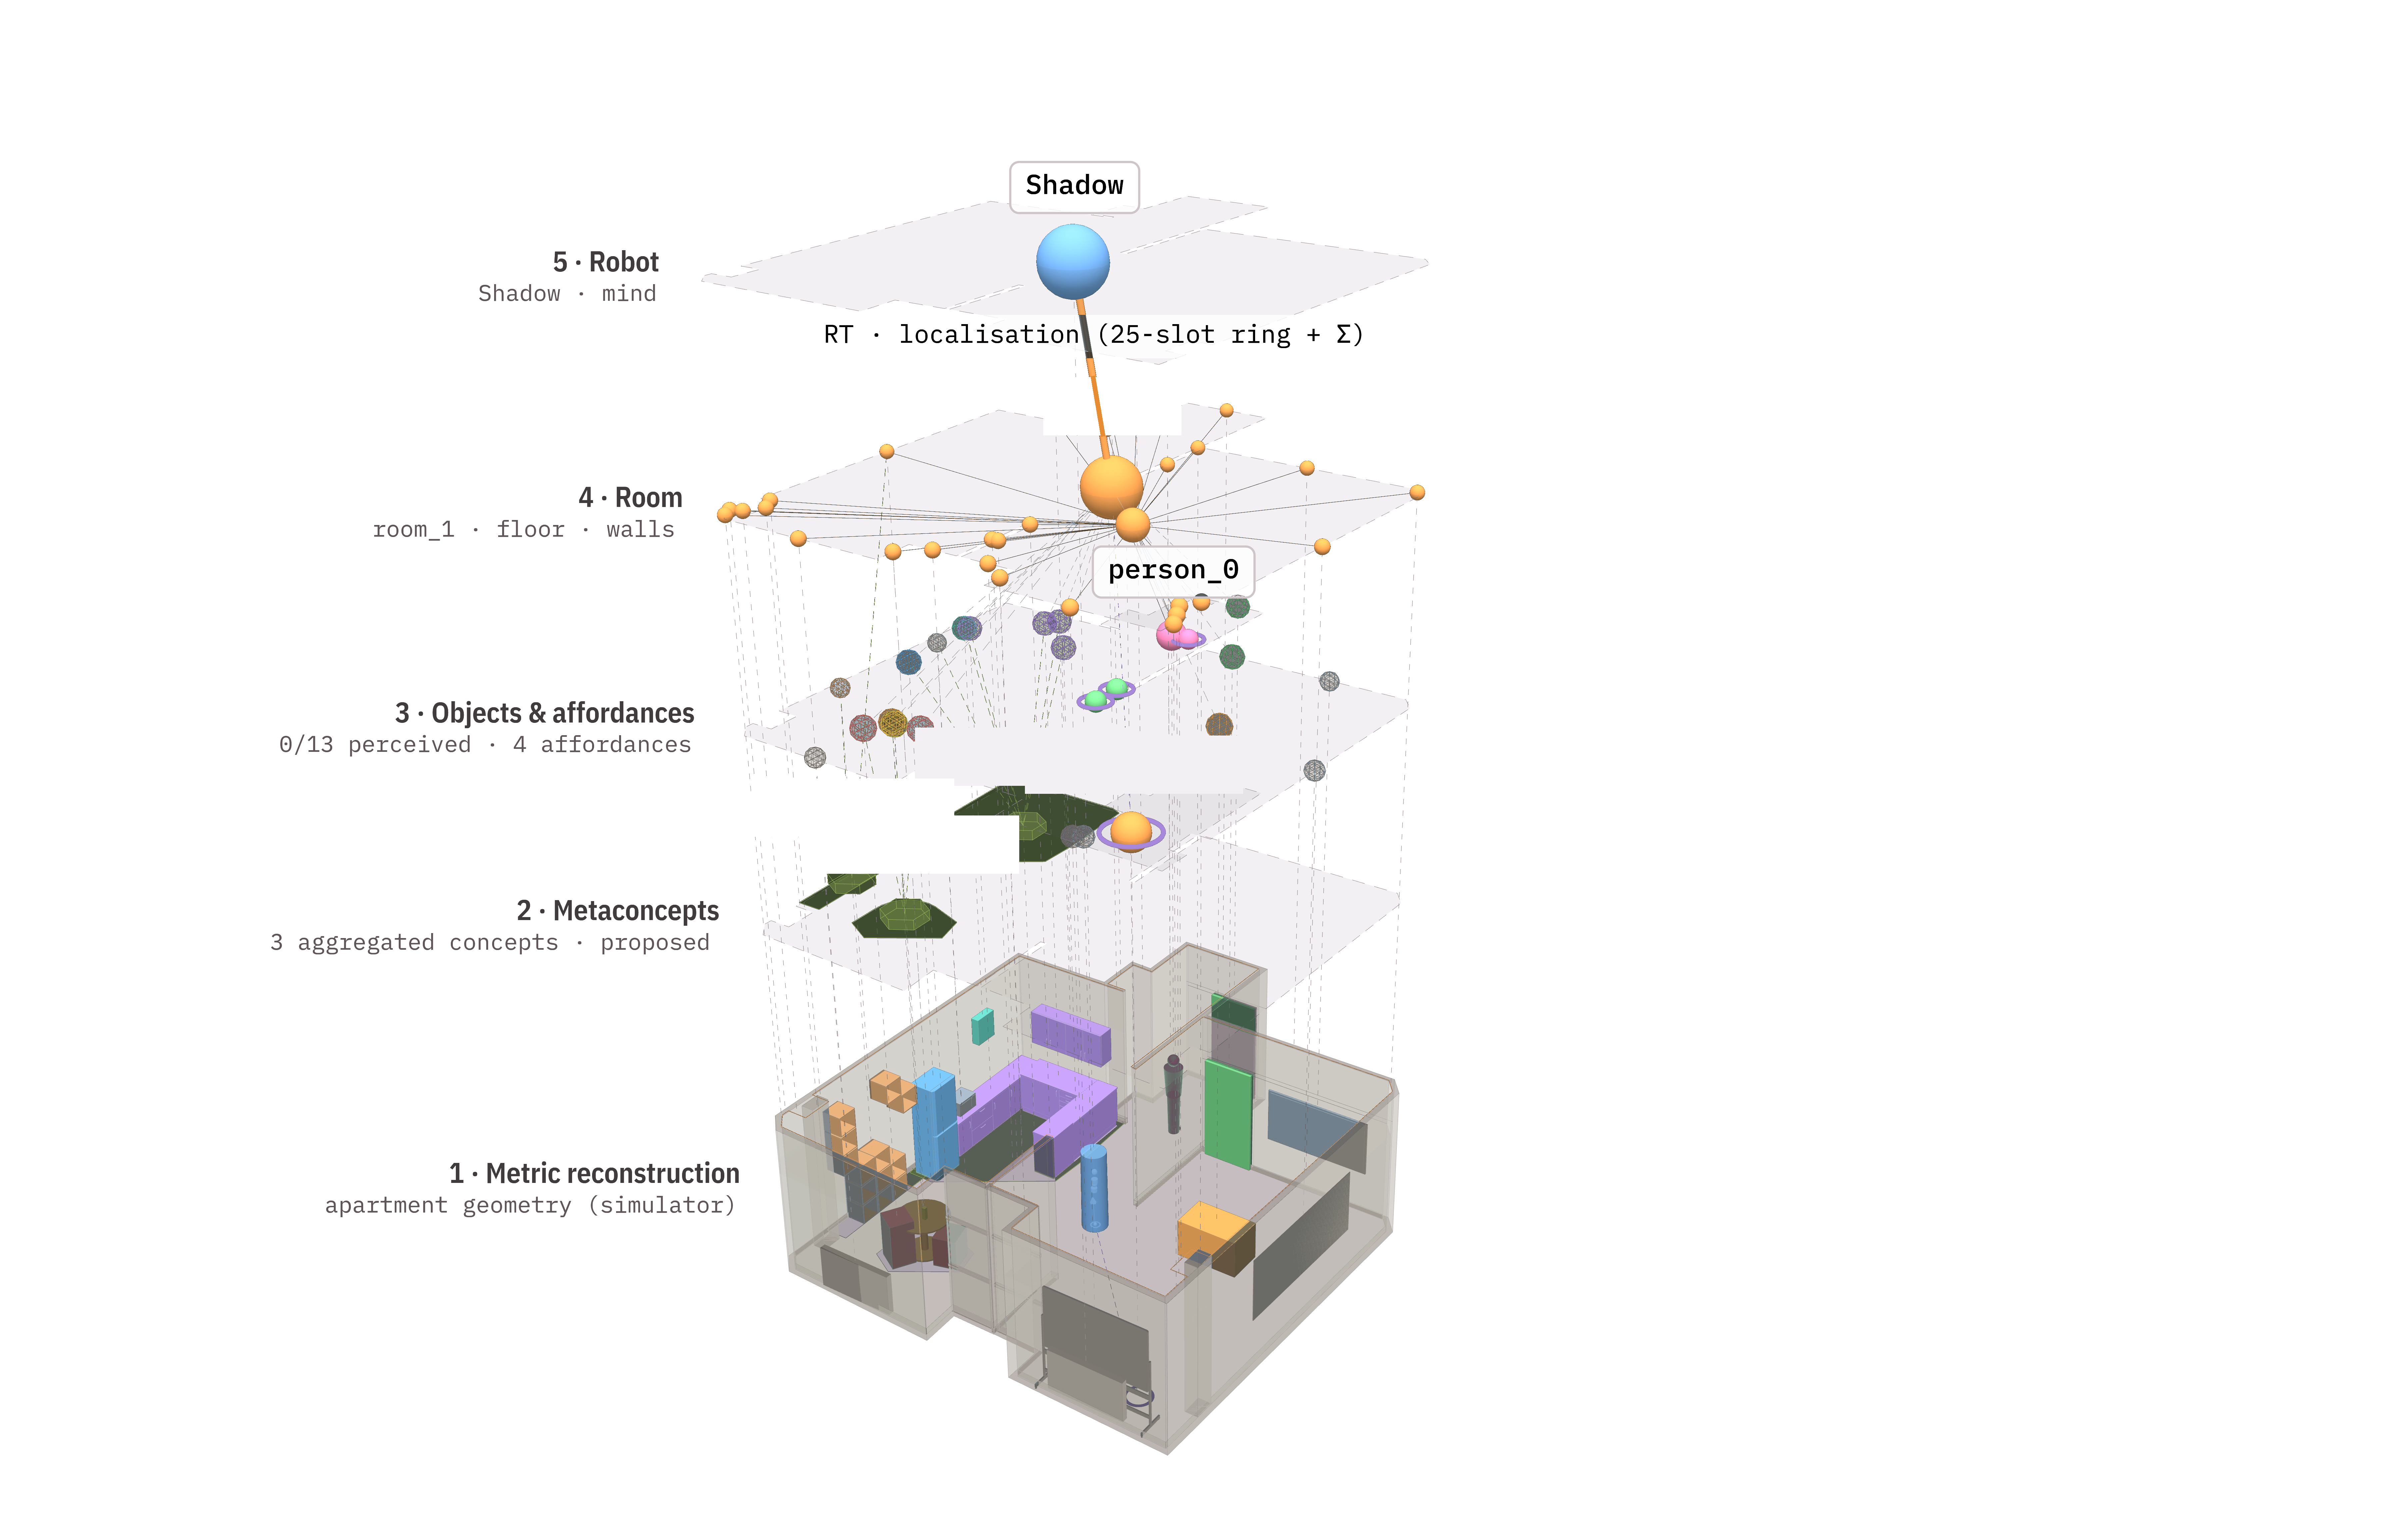
\includegraphics[width=\linewidth,trim=760 200 2850 420,clip]{figures/full_graph_white_clean.png}};
            \begin{scope}[x={(img.south east)}, y={(img.north west)}]
                % labels redrawn apart; the overlapping originals were removed from full_graph_white_clean.png
                \tikzset{lab/.style={draw=black!45, fill=white, rounded corners=1.5pt, inner sep=1.2pt,
                         font=\ttfamily\tiny}}
                \node[lab, anchor=east] at (0.690,0.800) {room\_1};
                \node[lab, anchor=west] at (0.425,0.505) {wall-shelf};
                \node[lab, anchor=west] at (0.470,0.462) {dinner-set};
                \node[lab, anchor=west] at (0.565,0.542) {kitchen-rig};
                \node[lab, anchor=west] at (0.775,0.515) {afford\_room};
                \fill[yellow!85!orange, draw=conceptc!80!black, thick] (0.80,0.585) circle (2.6pt);
                \node[draw=black!50, fill=white, rounded corners=1.5pt, inner sep=1.5pt,
                      font=\ttfamily\tiny, anchor=west] at (0.825,0.60) {chair\_34};
            \end{scope}
        \end{tikzpicture}
    \end{minipage}\hfill
    \begin{minipage}[c]{0.43\linewidth}
        \centering
        \resizebox{\linewidth}{!}{% belief-node.tex — schematic companion to Figure 2: one node of the graph as a belief.
% Uses the palette defined in vygotskian_machine_build.tex. Schematic, not data.
\begin{tikzpicture}[font=\scriptsize, >=Latex]
% ---------- the node card
\node[draw=conceptc, very thick, rounded corners=3pt, fill=conceptf, align=left, inner sep=4pt,
      text width=36mm, anchor=north west] (card) at (0,0) {%
  \tikz[baseline=-0.6ex]\fill[yellow!85!orange, draw=conceptc!80!black] (0,0) circle (2.4pt);\
  \textbf{\textcolor{conceptc!80!black}{chair\_34}}\\[1pt]
  owner: chair agent\\
  pose: mean $\mu$, covariance $\Sigma$\\
  existence: log-odds $\ell$\\
  parent: \texttt{room\_1}\\
  edge: transform $T$ and its $\Sigma$};
% ---------- floor sketch: pose belief seen from the robot
\begin{scope}[shift={(4.3,-2.15)}]
  \draw[black!55, thick] (0,0) -- (0,2.05) -- (3.0,2.05);
  \node[font=\tiny, text=black!55, anchor=south west] at (0,2.05) {room\_1 walls};
  % view cone
  \fill[wmc!25] (0.55,0.35) -- (2.75,1.65) -- (2.75,0.05) -- cycle;
  % robot
  \fill[bodyc!70] (0.55,0.35) circle (0.13);
  \draw[bodyc!80!black, thick, ->] (0.55,0.35) -- (0.9,0.55);
  \node[font=\tiny, text=bodyc!80!black, anchor=north] at (0.55,0.2) {robot};
  % chair belief: footprint at the mean, 2-sigma ellipse
  \draw[conceptc, thick, fill=conceptf, rotate around={25:(2.1,1.0)}] (2.1,1.0) ellipse (0.55 and 0.28);
  \draw[conceptc!80!black, fill=conceptc!45] (1.95,0.88) rectangle (2.25,1.12);
  \node[font=\tiny, text=conceptc!80!black, anchor=north] at (2.1,0.62) {$\mu$, $2\sigma$};
\end{scope}
% ---------- existence log-odds over time
\begin{scope}[shift={(0,-5.2)}]
  % segments
  \fill[wmc!18] (0.2,-0.75) rectangle (2.5,1.45);
  \fill[black!8] (2.5,-0.75) rectangle (4.6,1.45);
  \fill[bodyf] (4.6,-0.75) rectangle (7.0,1.45);
  \draw[->, black!60] (0,0) -- (7.35,0) node[anchor=west, font=\tiny, text=black!60] {time};
  \draw[->, black!60] (0,-0.75) -- (0,1.55) node[anchor=south, font=\tiny, text=black!60] {$\ell$};
  \draw[black!35, dashed] (0,0.0) -- (7.0,0.0);
  \draw[conceptc!85!black, very thick]
    (0.2,0.0) .. controls (0.9,0.7) and (1.6,1.05) .. (2.5,1.15)
    -- (4.6,1.15)
    .. controls (5.4,1.05) and (6.1,0.25) .. (6.9,-0.55);
  \node[font=\tiny, align=center, anchor=north] at (1.35,-0.78) {seen\\rises};
  \node[font=\tiny, align=center, anchor=north] at (3.55,-0.78) {occluded\\held};
  \node[font=\tiny, align=center, anchor=north] at (5.8,-0.78) {absent where\\detectable: falls};
\end{scope}
\end{tikzpicture}
}
    \end{minipage}
    \caption{Left: the output of \cortex{} in the simulated apartment, drawn by stratum: the robot (level~0),
    localised in \texttt{room\_1} (level~1); the objects and their affordances (level~2); and the aggregates fitted
    over them (level~3). The bottom stratum is the simulator's true geometry, shown for reference, and strata numbers
    give the drawing order, not the levels of Table~\ref{tab:lh_levels}. Right: a schematic of the node marked \texttt{chair\_34} on the left, as a belief
    owned by one agent, whose existence log-odds rises when the object is seen, is held while it is occluded, and
    falls only when it is absent where it could have been detected.}
    \label{fig:cortex_graph}
\end{figure}

\paragraph{Action and memory.}
A controller plans and follows paths. Its epistemic planner scores the actions that the concept agents offer, such as
looking at a door from a given place, by their expected free energy. An exploration drive turns this scoring into a
default behaviour. The robot explores the current room until further exploration yields too little information,
crosses the nearest uncrossed door, and returns in depth-first order. Three memory agents retain what the live graph
discards. The spatial memory stores each room the robot has left with the doors that connect it, and restores it as a
prior on return. The object memory keeps a persistent record of object instances. The episodic memory records the
robot's missions, their steps and how each ended. These memories provide the counts from which the priors and habits
of the Vygotskian machine will be learned.

\paragraph{The language agent.}
The language agent connects a person to all of these components through a vision-language model (VLM), Gemma 4
with 26 billion parameters, served by Ollama on an NVIDIA Jetson AGX Orin carried by the robot. Its design follows the principle
stated in the code as ``the model proposes, C++ decides''. The VLM sees a summary of the graph and the memories and can
act only by calling tools, and every call passes a deterministic gate that checks names against the graph and
arguments against the robot's capabilities. Extended behaviour is written in a small mission language (cross a door,
explore a room, approach an object, watch for a condition, if, repeat), and each mission is checked against the graph
and approved by the person before it runs. While a mission runs, robot events wake the model in restricted turns in
which it can look, query memory, stop and propose, but not act. Whether to ask the person or to make an assumption is
decided by a small rule over counts and costs. The agent also answers subjunctive questions with the robot's own
models, on an imagined copy of the room that can never write to the live graph. On that copy the controller answers
``would I fit?'', the perception models answer ``would I see it from there?'', and the episodic counts answer ``would
this route succeed?''. The imagination of Section~\ref{sec:lang_hierarchy:imagination} relies on these tools.

\paragraph{What is missing.}
\cortex{} can therefore perceive, hold beliefs, act, remember, talk and, when asked, imagine. Its VLM is used only when a
person speaks, nothing it knows becomes a prior, the robot never questions itself or imagines on its own initiative,
and the hundredth mission to the kitchen requires the same VLM calls as the first. The inner voice
(Section~\ref{sec:inner_speech}) and the cultural plane (Section~\ref{sec:lang_hierarchy}) address these gaps.
